%%==================================================
%% chapter03.tex for TJU Master Thesis
%% Encoding: UTF-8
%%==================================================

\chapter{基于粘声方程的反射全波形反演}

对于目前普遍缺乏可靠的低频(小于4Hz)以及长偏移距信息的地震数据,中深层的
参数信息主要包含在反射数据中,常规的FWI对于中深层参数的建模往往无能为力。
因此,反射波波形反演(RWI)成为近几年国际地震勘探领域争相研究的课题。沿
反射波波路径进行背景速度反演已经取得了很多成功的案例。

RWI是处理FWI的强非线性问题的一种有效解决途径,虽然在背景速度建模中被广泛
使用,但是目前为止,尚未有学者将其引入到背景$Q$的估计中。地震衰减对地震波传播
的影响相较于速度对地震波传播的影响既有相似之处,也略有不同。本章将详细介绍
如何把RWI引入到背景$Q$的反演中。

\vspace{0.5cm}
\section{引言}
\vspace{0.5cm}

用地震波信息来反演地下地层的衰减信息已有很多年的研究历史,其反演方法可大致
分为射线层析和波形反演两类。射线层析类方法(\citeA{brzostowski.mcmechan:1992};
\citeA{quan.harris:1997};\citeA{hu.liu:2011})用射线路径来构建层析矩阵,具有很高的
计算效率,对于介质变化简单的情况有很好的应用效果。但当介质复杂时,地震波传播往往
存在多路径,并且当介质存在高速或低速透镜体时,射线追踪会出现焦散现象,不能对其下覆
地层进行很好的照明。波动类的反演方法以全波动方程为传播引擎,能较精确的刻画地震波
在复杂介质中传播的各种波现象,理论上是目前精度最高的参数建模方法。自从
\citeB{lailly:1983}和\citeB{tarantola:1984}等人建立起全波形反演的基本理论框架以来,
越来越多的人关注该方法的研究与应用,尤其是在地震波速度反演方面。在地震品质因子
反演方面,\citeB{tarantola:1988}第一次提出了时间域粘弹波形反演理论。随后,
\citeB{song:1995}在频率域提出了一种粘声波形反演方法($Q$-FWI)。在$Q$-FWI中,速度
参数和品质因子有很强的耦合性(\citeA{song:1995};\citeA{kamei.pratt:2008};
\citeA{hak.mulder:2011})。在观测系统不完备的情况下,解决这中耦合性的思路有
两种,一种是通过预条件模型参数的梯度(\citeA{liao.mcmechan:1996};
\citeA{hak.mulder:2011};\citeA{malinowski:2011})来减弱耦合。另一种是顺序
反演法,先反演对地震数据影响较强的速度参数然后再反演$Q$模型(\citeA{pratt:2004};
\citeA{rao.wang:2008};\citeA{smithyman:2009})。

$Q$-FWI的成功需要低频长偏移距地震数据,但是这种高质量的数据采集需要高昂的采集费用。
当缺少长偏移距的折射数据时,深部模型往往只被反射波照明。因此,利用反射波进行中
深层的速度建模已成为地震成像的共识(\citeA{xu:2012a};\citeA{ma.hale:2013};
\citeA{chi:2015})。但是目前尚未有人用反射波波路径来进行地震衰减建模。本章
在顺序反演的思路下,先假设已获得准确的速度模型,然后引入RWI框架,用反射波来
反演背景$Q$模型。

\vspace{0.5cm}
\section{方法原理}
\vspace{0.5cm}
当利用反射波进行反演时,常规FWI对模型的短波长结构更敏感,而地震衰减对地震数据的
影响是一种沿地震波波路径的累加效应,因而,其长波长的背景模型显得更为重要。RWI通过
将数据残差投影到反射波波路径来构建模型的长波长成分,更加切合对地震衰减参数反演的
需求。本节将介绍粘声反射全波形反演($Q$-RWI)方法原理。

\vspace{0.5cm}
\subsection{反射波波形反演基本思路}
\vspace{0.5cm}
常规的FWI是通过匹配模拟数据和观测数据来推断介质的参数。设$\mathbf{x}_s$和$\mathbf{x}_g$
分别为炮点和检波点的空间位置,时间域FWI最常用的最小平方目标函数为(\citeA{virieux:2009}):
\begin{equation}
    \mathcal{J}(\mathbf{m})=\frac{1}{2}\sum_{s,g}\int_t[d_{obs}(\mathbf{x}_s,\mathbf{x}_g,t)
	        -d_{cal}(\mathbf{x}_s,\mathbf{x}_g,t)]^2dt,
	\label{eq:misfit_function}
\end{equation}
其中$d_{cal}(\mathbf{x}_s,\mathbf{x}_g,t)$是模拟数据,$d_{obs}(\mathbf{x}_s,\mathbf{x}_g,t)$
是观测数据。将目标函数(方程~\ref{eq:misfit_function})在$\mathbf{m}_0$附近进行二阶Taylor展开
有
\begin{equation}
	\mathcal{J}(\mathbf{m}_0+\Delta\mathbf{m})=\mathcal{J}(\mathbf{m}_0)
	+\frac{\partial\mathcal{J}(\mathbf{m}_0)}{\partial\mathbf{m}}\Delta\mathbf{m}
	+\frac{\partial^2\mathcal{J}(\mathbf{m}_0)}{\partial\mathbf{m}^2}\Delta\mathbf{m}^2 
	+ \mathcal{O}(\Delta\mathbf{m}^3).
\end{equation}
当目标函数对模型参数在$\mathbf{m}_0$处的一阶导数等于零时,目标函数取得极小值,即
\begin{equation}
	\Delta\mathbf{m}=-[\frac{\partial^2\mathcal{J}(\mathbf{m}_0)}{\partial\mathbf{m}^2}]^{-1}
	\frac{\partial\mathcal{J}(\mathbf{m}_0)}{\partial\mathbf{m}},
\end{equation}
式中$\frac{\partial\mathcal{J}(\mathbf{m}_0)}{\partial\mathbf{m}}$为梯度方向,$[\frac{\partial^2
\mathcal{J}(\mathbf{m}_0)}{\partial\mathbf{m}^2}]^{-1}$为Hessian的逆。Hessian的逆对反演通常起
照明补偿、加快收敛的作用,但是其计算非常困难,在反演中通常对其做对角近似或常数近似。而一阶梯度
作为目标函数的下降方向显得尤为重要。根据伴随状态法(\citeA{plessix:2006}),目标函数的梯度可用
正传波场与反传的残差波场进行零延迟的互相关得到,即
\begin{equation}
	\frac{\partial\mathcal{J}(\mathbf{m}_0)}{\partial\mathbf{m}} = \mathbf{\lambda}\otimes\mathbf{u},
\end{equation}
其中$\otimes$表示零延迟互相关,$\mathbf{\lambda}$,$\mathbf{u}$分别表示伴随波场和正传波场。
图~\ref{fig:grad_full}展示了两层介质单炮单检波点的常规FWI梯度。其梯度包含四个不同的子梯度
(图~\ref{fig:grad}),
直达波梯度、源端反射波梯度、检波点端反射波梯度以及偏移响应。从图中可以看出不同类型的波
对梯度的贡献量不一样,假设透射波场的振幅为1,背向的反射波的振幅为反射系数的量级$R$(譬如0.1)。
那么梯度中,透射波贡献的能量最强(图~\ref{fig:grad}a),将折射波的数据沿透射波波路径反投影
就可以很好地更新折射波波路径覆盖区域的背景参数,但是这部分能量在深层为零。在FWI的初期阶段
中不合需要的分量是偏移响应(图~\ref{fig:grad}b),其强度为$R$,是由反射波沿折射波波路径投影
得到的。而反演中深部背景参数需要令反射波沿着类似透射形状的反射波路径进行背景参数更新
(图~\ref{fig:grad}c和d),其中兔耳状反射波梯度的强度仅为$R^2$。因此,最需要的兔耳状的
反射波梯度比不合需要的偏移响应的强度还要小一个数量级,如果不采用梯度分解,需要的低波数
能量会被不需要的高波数偏移响应所掩盖,这就是常规FWI通常难以用反射波来更新背景参数的最
主要原因。

\begin{figure*}[!htbp]
	\centering
	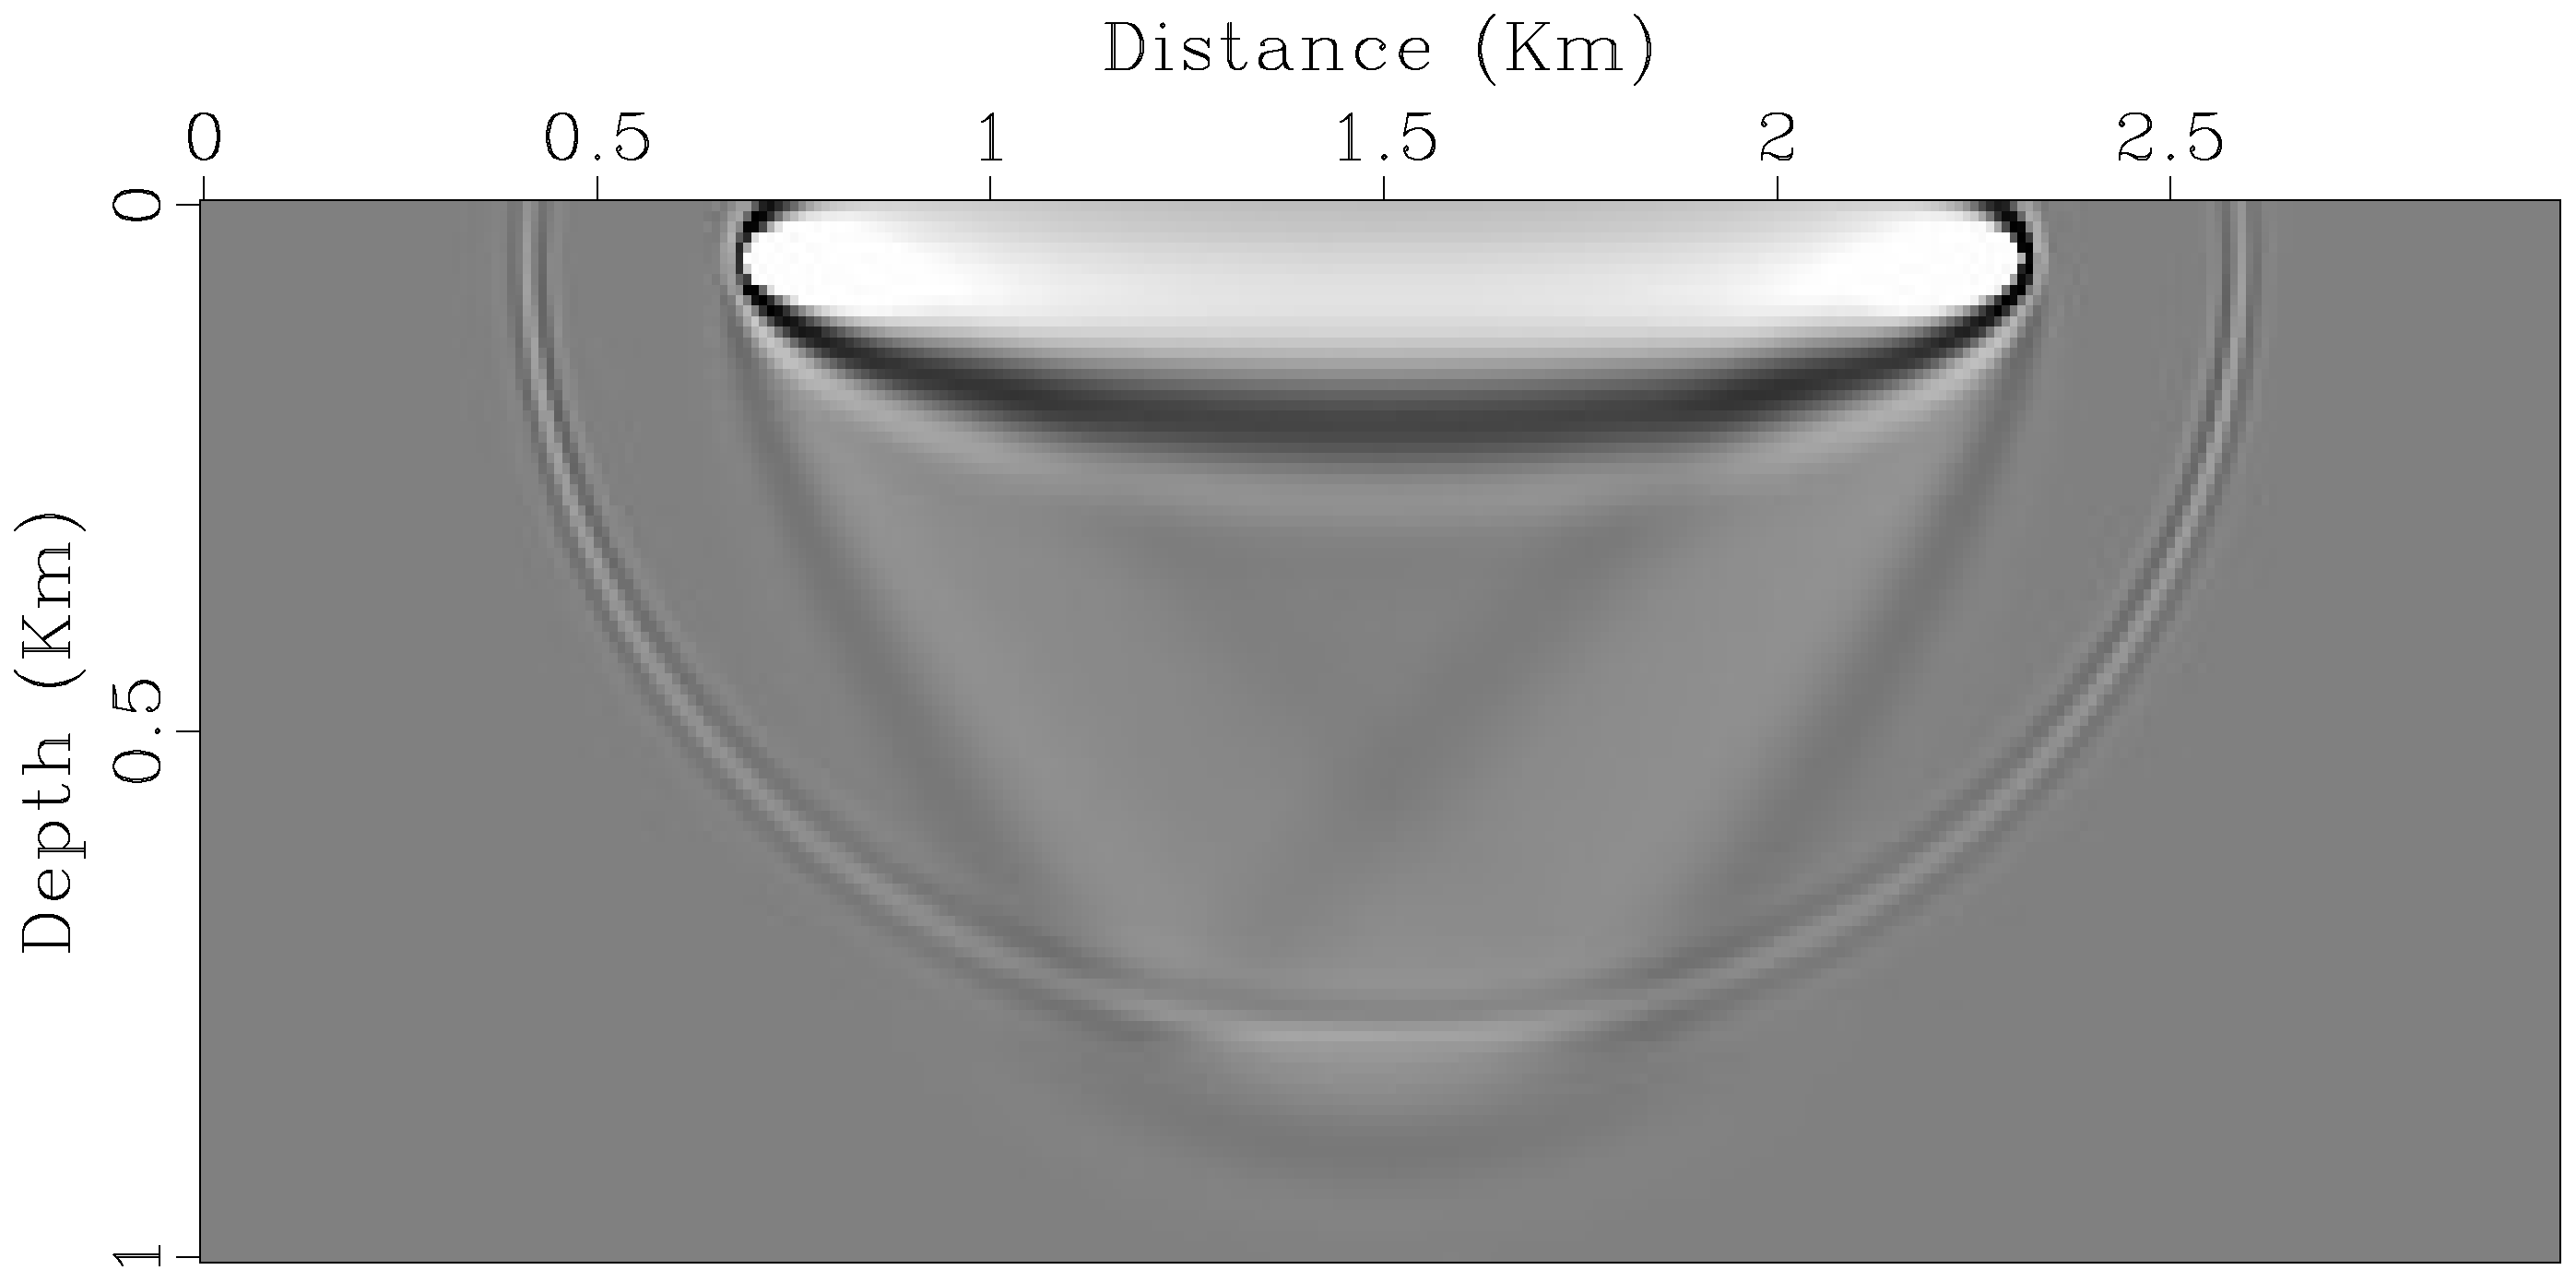
\includegraphics[width=0.95\linewidth]{figure/grad_full}
	\fcaption{两层介质单炮单检波点的FWI梯度。}{The gradient of FWI.
	 }[常规FWI梯度]
	\label{fig:grad_full}
\end{figure*}

\begin{figure*}[!htbp]
	\centering
	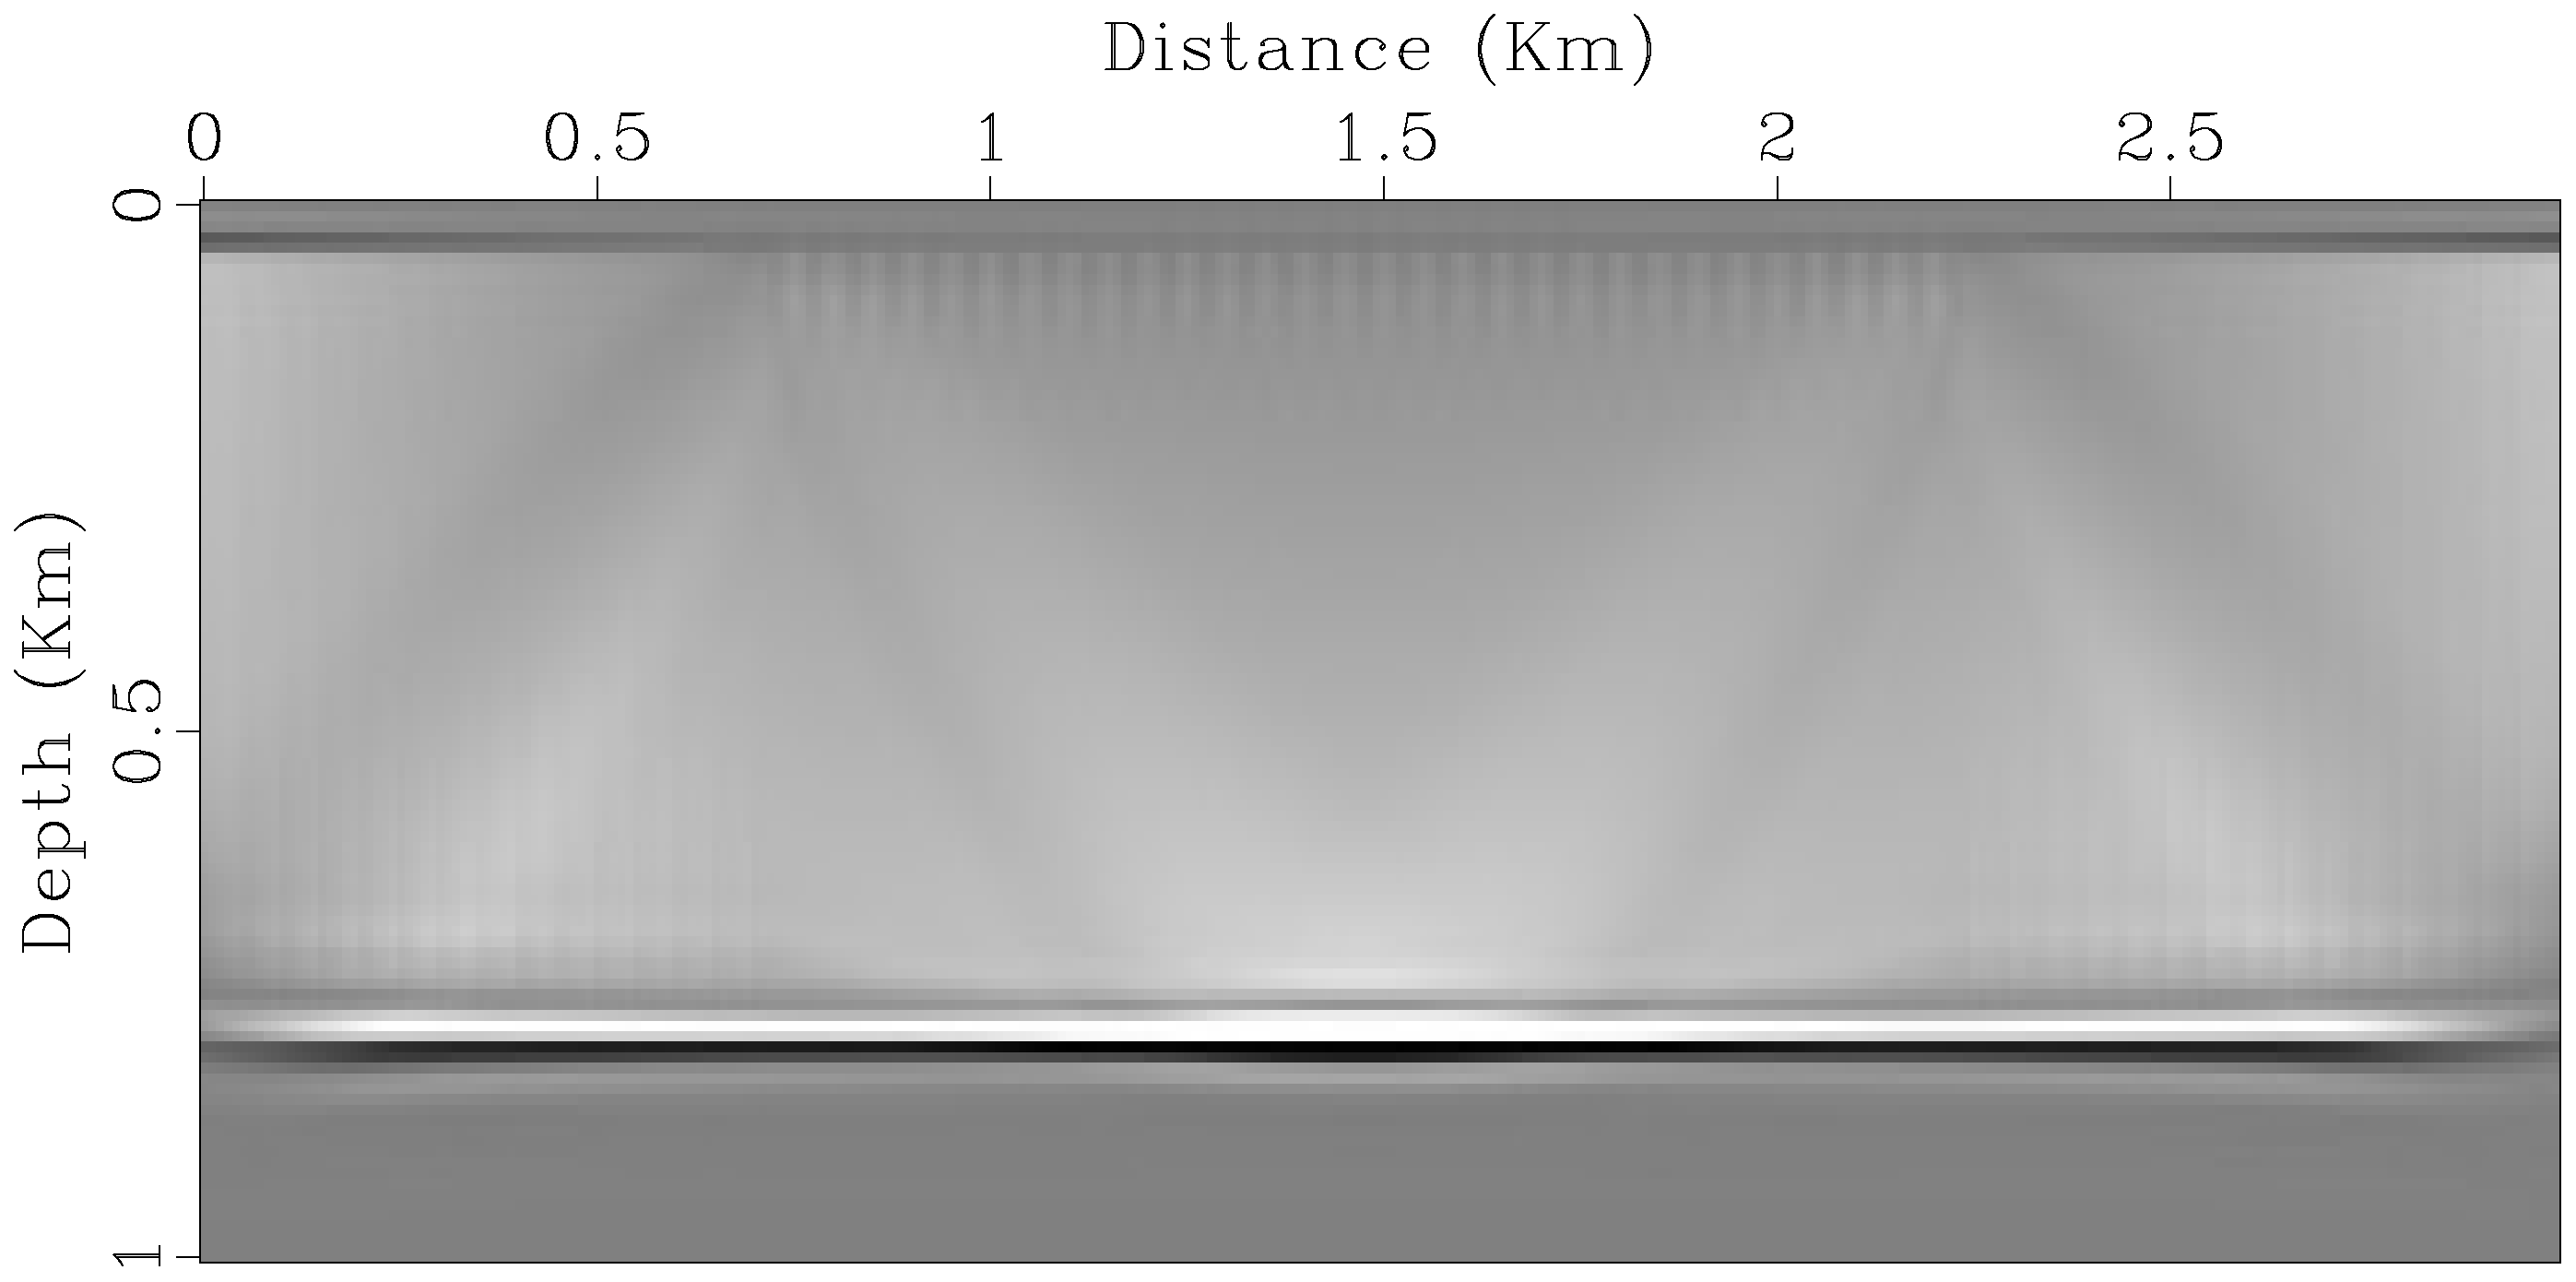
\includegraphics[width=1.0\linewidth]{figure/grad}
	\fcaption{常规FWI梯度分解。(a)直达波梯度;(b)偏移响应;(c)源端反射波梯度;
	(d)检波点端反射波梯度。}{The sub-gradients of FWI. (a) direct wave gradient; 
	(b) migration-ellipse; (c) source side gradient; (d) receiver side gradient.
	 }[常规FWI梯度分解]
	\label{fig:grad}
\end{figure*}

RWI主要是通过上下行波分离来提取反射波在反射波路径上的梯度。目前在RWI中用于上下行波分离
的方法主要两种,一种是在光滑的背景模型中加入参数扰动,用Born正演来获取上行的反射波
(\citeA{xu:2012a};\citeA{ma.hale:2013};\citeA{chi:2015});另一种是在频率-波数域
用方向分解来区分上下行波(\citeA{wang:2016})。另外,单成波方程自然地考虑了波的传播
方向,非常适合RWI的框架,已逐渐开始被学者用于RWI的研究中(\citeA{dong:2018})。
本节将用基于Born正演的方式来重述RWI的推导。

根据\citeB{ma.hale:2013}的推导,将模型参数$\mathbf{m}$分解为光滑的低波数背景模型
$\mathbf{m}^s$和高波数扰动$\mathbf{m}^r$(图~\ref{schematic_rwi}):
\begin{equation}
	\mathbf{m}=\mathbf{m}^s+\mathbf{m}^r.
\end{equation}
其中光滑的背景参数$\mathbf{m}^s$控制波传播的运动学信息,即背景波场$\mathbf{p}_b
\equiv p_b(\mathbf{x}_s,\mathbf{x}_g,t)$:
\begin{equation}
	\left(\mathbf{m}^s\frac{\partial^2}{\partial t^2}-\bigtriangledown^2\right)\mathbf{p}_b
	=f(t,\mathbf{x}_s),
\end{equation}
高波数扰动$\mathbf{m}^r$对应于反射波场$\mathbf{p}_c\equiv p_c\mathbf{x}_s,\mathbf{x}_g,t)$:
\begin{equation}
	\left((\mathbf{m}^s+\mathbf{m}^r)\frac{\partial^2}{\partial t^2}-\bigtriangledown^2\right)
	\mathbf{p}_c=-\mathbf{m}^r\frac{\partial^2}{\partial t^2}\mathbf{p}_b,
\end{equation}
式中$\mathbf{m}^r$和$\mathbf{m}^s$是慢度的平方,$f(t,\mathbf{x}_s)$表示震源子波。

\begin{figure*}[!htbp]
	\centering
	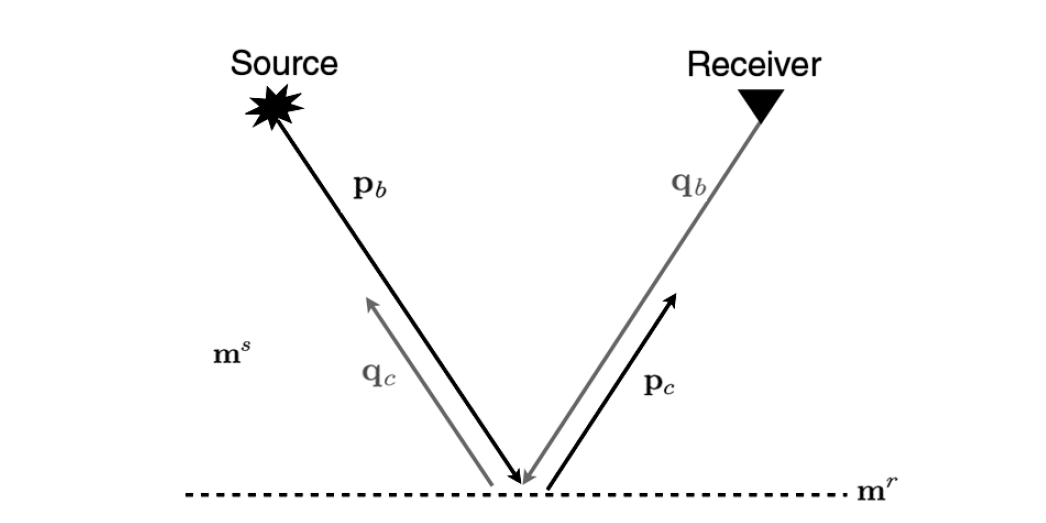
\includegraphics[width=0.7\linewidth]{figure/schematic_rwi}
	\fcaption{RWI波场分解及波路径示意图,参数的高波数成分($\mathbf{m}^r$)扰动背景场
	$\mathbf{p}_b$和$\mathbf{q}_b$产生背向散射场$\mathbf{p}_c$和$\mathbf{q}_c$,可以看作
	是”透射波“从震源出发沿波路径到达反射位置$\mathbf{m}^r$然后再返回接收点。}
	{Schematic of RWI. The high-wavenumber component
	$m^r$ perturbs wavefields $\mathbf{p}_b$ and $\mathbf{q}_b$ in the
	low-wavenumber background $m^s$ and contributes to back-scattering
	wavefields $\mathbf{p}_c$ and $\mathbf{q}_c$, which can be considered
	“transmission” waves propagating along the wave paths between $m^r$ and
	the source and receiver.}[RWI波场分解及波路径示意图]
	\label{fig:schematic_rwi}
\end{figure*}

\vspace{0.5cm}
\subsection{基于粘声方程的反射全波形反演}
\vspace{0.5cm}

\section{数值实验}

